\documentclass{article}
\setlength\topmargin{0pt}
\addtolength\topmargin{-\headheight}
\addtolength\topmargin{-\headsep}
\setlength\oddsidemargin{0pt}
\setlength\textwidth{\paperwidth}
\addtolength\textwidth{-2in}
\setlength\textheight{\paperheight}
\addtolength\textheight{-2in}
\usepackage{layout}
\usepackage{amsmath}
\usepackage{algorithm}
\usepackage{verbatim}
\usepackage[noend]{algpseudocode}
\usepackage{graphicx}
\graphicspath{ {./} }


\title{\vspace{-2.0cm}CS M152A Project 4 Report}
\author{Melody Chen}

\begin{document}
\maketitle
\section{Introduction and Requirement} 
The focus of this lab is for students to learn about how to design finite state machine that matches the specified behavior and to use the Xilinx ISE software to design and test state machines. Finite State Machines (FSMs) are used in many real world systems. An FSM has a finite number of states and can be in one state at a given time. There are two types of FSM machines: Moore Machine and Mealy Machine. A Moore machine's output only depends on which state it is in, but a Mealy machine's output depends on both the current state and input. For this assignment, we're tasked with designing a vending machine with the following characteristics:
\begin{enumerate}
    \item Vending machine has 20 different snacks for sale. Each snack has two digit code (00 to 19).
    \item Each snack is stored in separate slot. There can be up to 10 units of snack stored in 1 slot.
    \item A buyer can purchase only 1 item at a time. 
    \item The machine only accepts payment by card. 
\end{enumerate}
\begin{center}
    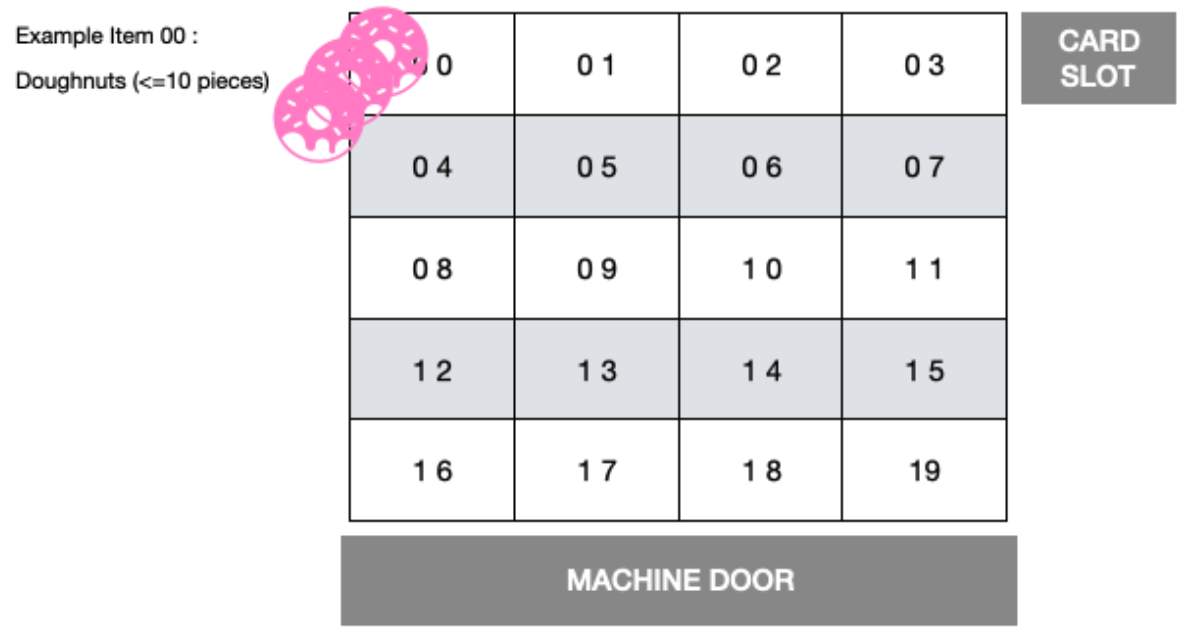
\includegraphics[scale=0.5]{intro.png} \\
    \caption{Vending Machine Figure from Manuscript}
\end{center} 
More details about specific behaviors of our vending machine FSM will be covered in the next sections.


\section{Design Description}
For the design and implementation of the varying types of FSM, I followed guidance provided in the project specifications.  I first consider the inputs provided and what my FSM will need to output. Our Vending Machine FSM will be given the following inputs, and we will need to output specific values for the outputs shown in the diagram below: 
\begin{center}
    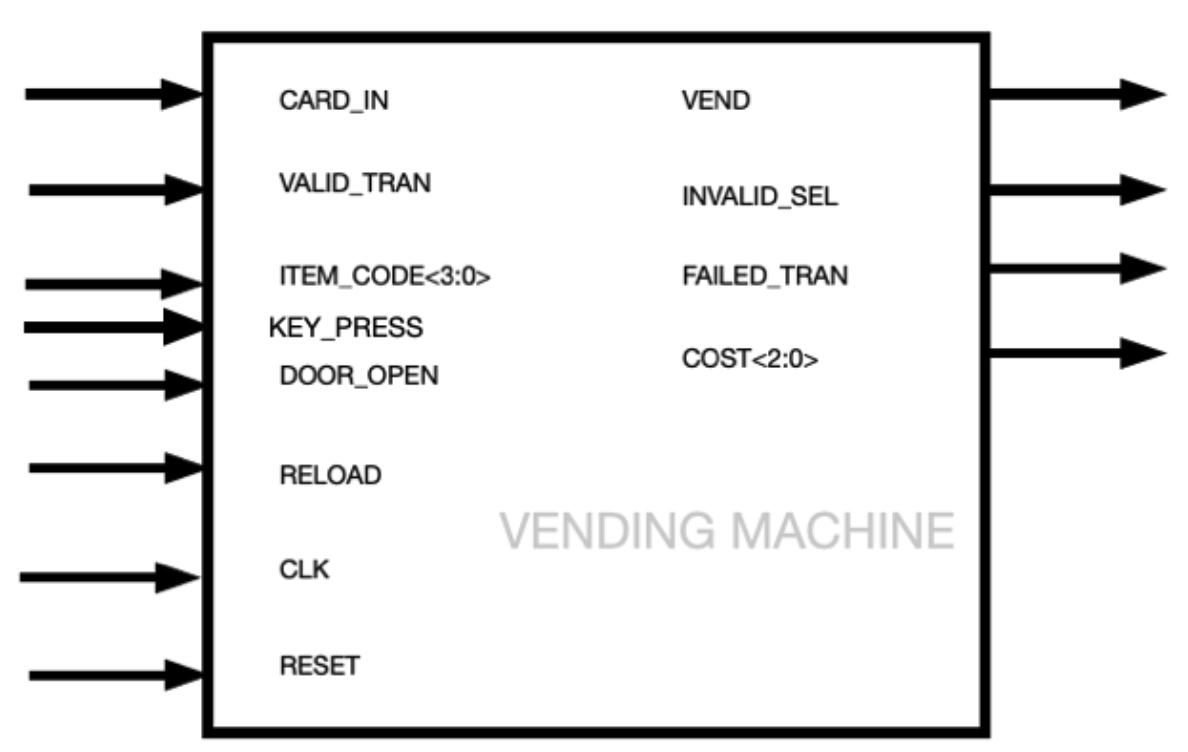
\includegraphics[scale=0.4]{input_outputs.png} \\
    \caption{Vending Machine I/O from Manuscript}
\end{center} 
I then designed my FSM with around 10 states that correctly captures the behavior described in the manuscript. My FSM is a Moore machine, meaning that my output depends only on which state I am in, regardless of the inputs. 
\begin{center}
    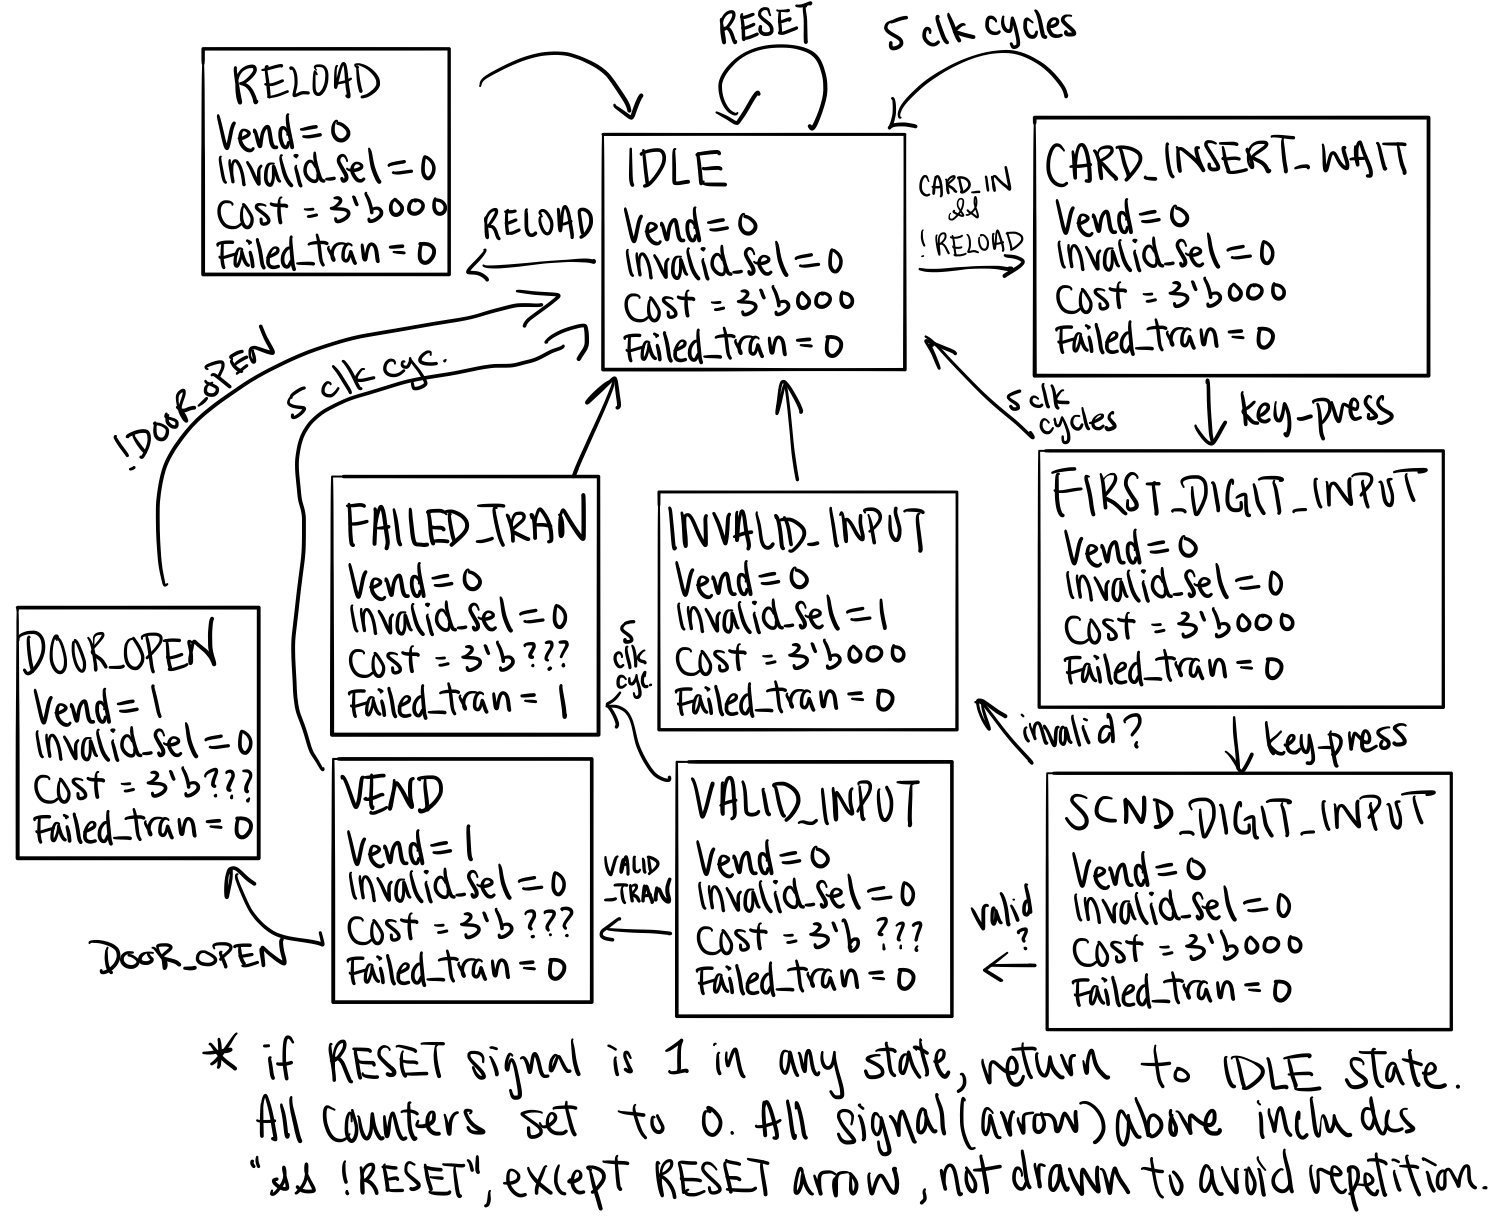
\includegraphics[scale=0.25]{FSM-diagram.jpeg} \\
    \caption{Moore FSM Design of Vending Machine}
\end{center} 
Descriptions of states and transitions of above FSM:
\begin{itemize}
    \item Once \texttt{RESET} signal is 1, we will begin at the IDLE state, where our Vending Machine waits for the \texttt{RELOAD} or \texttt{CARD\_IN} signal to be 1. All outputs should be 0, including count of items inside vending machine. This represents the state where no one is using our vending machine yet.
    \item Once \texttt{RELOAD} signal is 1, we transition to the RELOAD state where all our outputs remain unchanged, but the internal count for each slot in the vending machine should be set to 0. Once counts are set to 0, we directly return to IDLE state.
    \item From the IDLE state, when \texttt{RELOAD} signal is 0, and \texttt{CARD\_IN} signal is 1, we transition into the CARD\_INSERT\_WAIT state. Outputs remain all zeroes. 
    \item In CARD\_INSERT\_WAIT state, we wait for either 5 clock cycles to pass and transition back to the IDLE state or \texttt{KEY\_PRESS = 1} and transition to FIRST\_DIGIT\_INPUT state.  After 5 cycles has passed, this represents our vending machine not receiving any code entered. When we detect a key press, we want to transition to next state where we prepare to read in a second key press.
    \item In FIRST\_DIGIT\_INPUT state, all our outputs remain 0. We check if 5 clock cycles has passed and return to the IDLE state, or we check \texttt{KEY\_PRESS = 1} and transition to SCND\_DIGIT\_INPUT state. 
    \item In SCND\_DIGIT\_INPUT state, all our outputs remain 0. We have detected two different \texttt{ITEM\_CODE}, so we have check whether the code represents a valid input. If the number falls between 00-19 and the item is still available, we transition to the VALID\_INPUT state. Otherwise, we transition to the INVALID\_INPUT state. 
    \item In INVALID\_INPUT state, we output \texttt{INVALID\_SEL = 1} and return to IDLE\_STATE.
    \item In VALID\_INPUT state, we output the \texttt{COST} corresponding to the valid input numbers, and rest of outputs remain 0. After 5 clock cycles, if \texttt{VALID\_TRAN} remains 0, we transition to the FAILED\_TRAN state. If \texttt{VALID\_TRAN = 1} within 5 cycles, we transition to the VEND state. This signifies the the card payment was accepted. 
    \item In FAILED\_TRAN state, we output \texttt{FAILED\_TRAN = 1}, cost of item selected, and rest of outputs remain 0. We then return to the IDLE state in the next clock cycle.
    \item In VEND state, we output cost of item and \texttt{VEND = 1}. Rest of outputs remain 0. We wait 5 clock cycles for \texttt{DOOR\_OPEN} to be 1 to transition into the DOOR\_OPEN state. If door remains closed for 5 cycles, we return to IDLE state.
    \item In DOOR\_OPEN state, we continue to output cost of item, \texttt{VEND = 1}, and rest of outputs are 0. We wait for \texttt{DOOR\_OPEN = 0} to transition to IDLE state, signifying end of our transaction. We remain in this state until  \texttt{DOOR\_OPEN = 0} or we receive the reset signal. 
    \item Note: If \texttt{RESET = 1} at any point in our state diagram, it overrides other signal and arrows, reset all counts in vending machine to zero, and transitions to IDLE. 
\end{itemize}
To implement the above FSM in Verilog, I created the \texttt{vending\_machine} top module that takes in input listed in the Vending Machine I/O Diagram and outputs the outputs shown in the same diagram. Within my module, I initialized parameters representing all the states I have with a unique 4 bit binary number, two 4-bit registers \texttt{current\_state} and \texttt{next\_state}, and 20 4-bit registers corresponding to the count for each item in the vending machine. I have 3 main always block each with a specific task, similar to the sample code provided in the manuscript:
\begin{enumerate}
    \item Sequential always block to update \texttt{current\_state} to \texttt{next\_state} at every \texttt{posedge} of the clock or update \texttt{current\_state} to IDLE state when \texttt{RESET = 1}.
    \item Combinational always block to decide what \texttt{next\_state} should be based on the current state and current inputs.
    \item Combinational always block to decide what outputs should be based on the current state and values stored in registers from inputs, such as which item is selected.
\end{enumerate}
Aside from the blocks mentioned above, I have two more sequential always block that helps me with counting when 5 cycles has passed once we enter a particular state, such as CARD\_INPUT\_WAIT state. One always block uses a counter we implemented in previous projects and the other always block is in charge of setting a signal \texttt{clk\_start} to signify that counter should start counting up. 
\begin{center}
    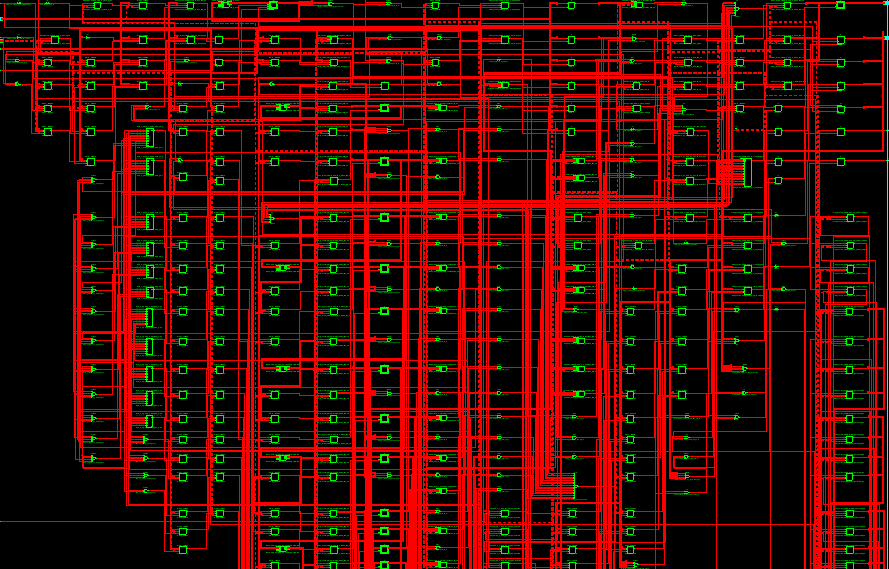
\includegraphics[scale=0.4]{rtl-lab4.png} \\
    \caption{RTL Schematic of Vending Machine FSM}
\end{center} 
From first look, the RTL schematic above looks filled with registers, muxes, and counters. This makes sense as our FSM is fairly complicated having to keep track of 20 registers for each item in our vending machine on top of keeping track of the combinational logic to calculate the next state and the outputs. My Verilog code results in this schematic being generated as my code has 2 large combinational logic sections and requires many registers to keep track of internal signals to calculate the outputs and the next state.
\section{Simulation Documentation}
To test whether the FSM I implemented works as the manuscript described, I created my testbench that tests not only the successful runs of ordering an item from the vending machine, but all of the possible special cases, such as no key is pressed or an item has ran out. To simulate behavior of someone interacting with the vending machine, in my testbench, I created a system clock with T=10ns, and at each negative edge I change a particular input to observe how my FSM will deal with the change in input. Below are all the different cases I tested and their respective waveform.
\begin{enumerate}
    \item \textbf{Successful Purchase of Valid In-Stock Item} \\
    This case represents a successful purchase from the vending machine machine where there were no errors all the way until vending machine door closes. The last light blue wave in the diagram below is an extra waveform I chose to display as output in order to show transition from one state to another. It is the binary representation of which state we're in. The way I simulated this behavior in the test bench is by first setting \texttt{RESET} as high to initialize all outputs to 0 and transition to the IDLE state. I then set \texttt{RELOAD = 1} in order to fill up the vending machine with stocks(shown at 70ns). Now to simulate someone using the machine, I set input \texttt{CARD\_IN = 1} (shown at 110ns) and we're now in state \texttt{4'b0010} CARD\_INSERT\_WAIT state. So far all output remains 0 as no mistakes has occurred and nothing has been inputted yet. We then set \texttt{KEY\_PRESS} to high twice in the next 3 cycles in order to simulating pressing keys 1 and 3 into the machine(130ns-200ns). At 200ns, we transition into state \texttt{4'b0110} VALID\_INPUT as 13 corresponds to a valid in stock item in our machine. We correctly see that output \texttt{COST = 4} at 200ns and beyond, since from the manuscript cost of item 13 is 4. We then set \texttt{VALID\_TRAN = 1} to represent the acceptance of our payment and once this signal is process we see that output \texttt{VEND = 1}. At 230ns, we set \texttt{DOOR\_OPEN = 1} for one cycle to simulate item coming out of the machine. Once \texttt{DOOR\_OPEN = 0} at 250ns, we see that \texttt{COST = 0} and \texttt{VEND = 0} as we have returned to IDLE state, which is the correct behavior.
    \begin{center}
        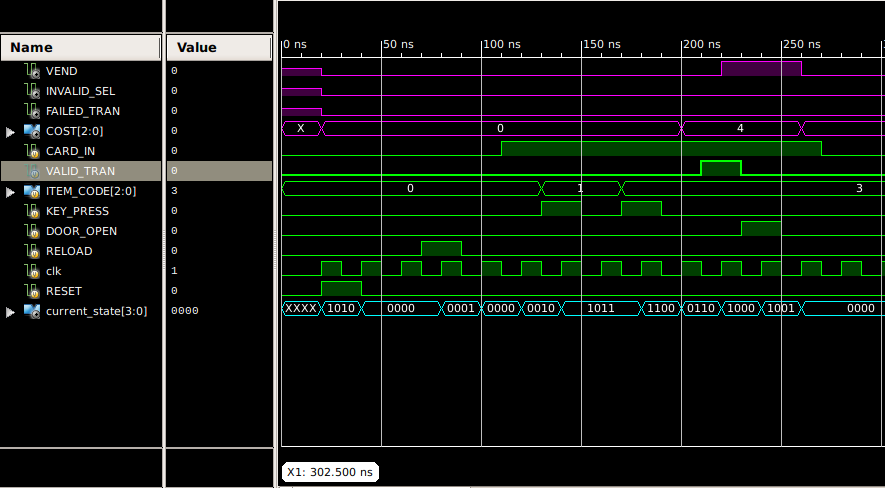
\includegraphics[scale=0.5]{waveform-1.png} \\
        \caption{Simulation Waveform for Case 1}
    \end{center}
    \par
    
    \item \textbf{Unsuccessful Purchase, No Key Press Detected}\\
    This case represents an unsuccessful purchase where we return to IDLE state as after 5 clock cycles, no key press is detected. To simulate this case, we simply set \texttt{CARD\_IN = 1} to transition into state \texttt{4'b0010} CARD\_INSERT\_WAIT and observe what happens after 5 clock cycles. At 320ns, we enter CARD\_INSERT\_WAIT, where all outputs are 0, and at 420ns, we see \texttt{INVALID\_SEL = 1} for one cycle. One cycle is 20ns, thus our FSM correctly waits for 5 cycles before entering \texttt{4'b0101} INVALID\_INPUT state, and outputting \texttt{INVALID\_SEL = 1}. After one cycle, we return to IDLE state where all output is 0. Thus, our FSM behaves as described by the manuscript in this edge case.
    \begin{center}
        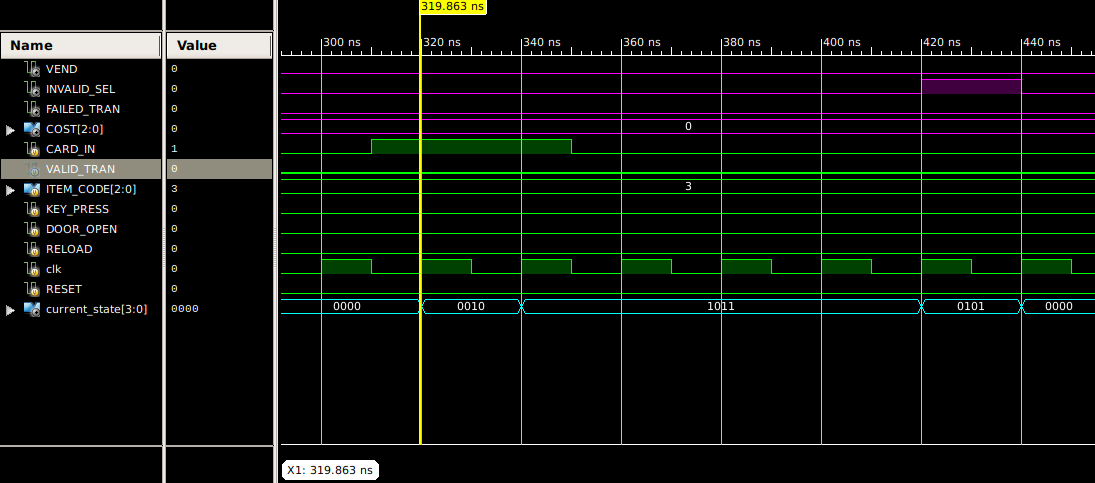
\includegraphics[scale=0.4]{waveform-2.png} \\
        \caption{Simulation Waveform for Case 2}
    \end{center}  \par

    \item \textbf{Unsuccessful Purchase, Only 1 Key Press Detected}\\
   This case represents an unsuccessful purchase where we return to IDLE state as we detect 1 key press, but after 5 cycles, we do not detect a second key press. To simulate this case, we simply set \texttt{CARD\_IN = 1} to transition into state \texttt{4'b0010} CARD\_INSERT\_WAIT, we then set \texttt{KEY\_PRESS = 1} for one cycle, and observe what happens after 5 clock cycles. At 580ns, we detected and registered the first key press, all outputs remain 0 and we begin our counter. At 680ns, we see \texttt{INVALID\_SEL = 1} for one cycle. One cycle is 20ns, thus our FSM correctly waits for 5 cycles before entering \texttt{4'b0101} INVALID\_INPUT state, and outputting \texttt{INVALID\_SEL = 1}. After one cycle, we return to IDLE state where all output is 0. Thus, our FSM behaves as described by the manuscript in this edge case.
    \begin{center}
        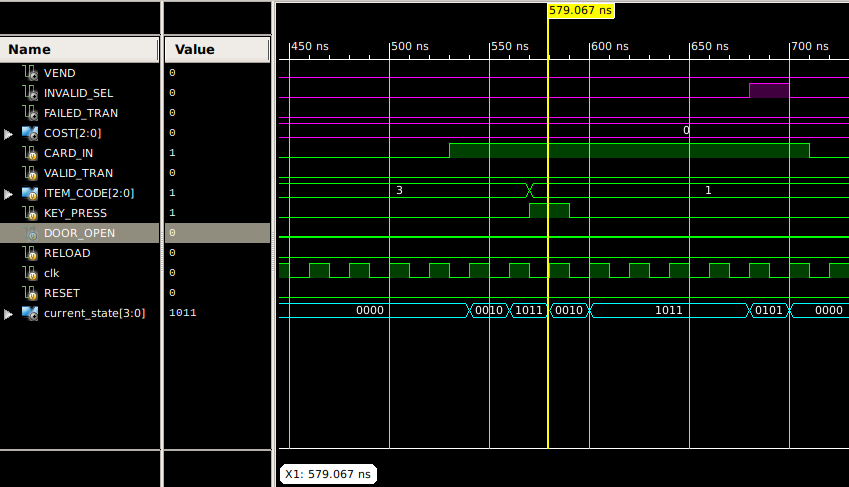
\includegraphics[scale=0.5]{waveform-3.png} \\
        \caption{Simulation Waveform for Case 3}
    \end{center}
    \par
    
    \item \textbf{Unsuccessful Purchase, Out of Range Item Number Entered}  \\
    This case represents an unsuccessful purchase where two key press are detected, but the number they represent is out of range, so we want \texttt{INVALID\_SEL = 1}. To simulate this case, we simply set \texttt{CARD\_IN = 1} to transition into state \texttt{4'b0010} CARD\_INSERT\_WAIT, we then set \texttt{KEY\_PRESS = 1} for one cycle, and then set \texttt{KEY\_PRESS = 1} for one cycle. The two keys we entered are 2, 7, representing an item that doesnt exist in our vending machine. At 760ns, we see that 2 is read by our FSM, and then at 800ns, 7 is read by our FSM. One cycle after 7 is read, we see that at 820ns, \texttt{INVALID\_SEL = 1} for one cycle. This is the correct behavior as 27 is an invalid input.
    \begin{center}
        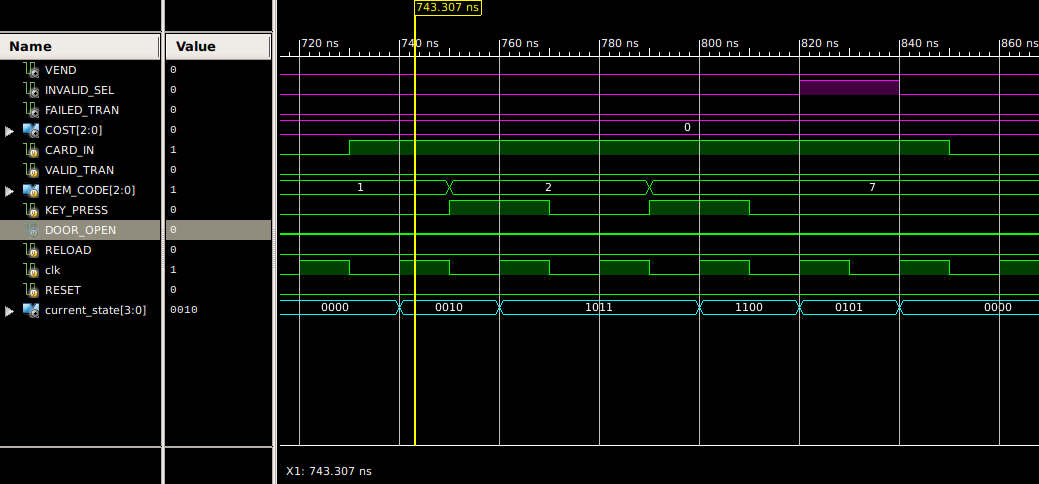
\includegraphics[scale=0.4]{waveform-4.png} \\
        \caption{Simulation Waveform for Case 4}
    \end{center}

    \item \textbf{Unsuccessful Purchase, Invalid Transaction}  \\
    This case represents an unsuccessful purchase where valid keys are inputted and the item requested has stock, but our card transaction has failed. To simulate this case, we set \texttt{CARD\_IN = 1} to transition into state \texttt{4'b0010} CARD\_INSERT\_WAIT, we then set \texttt{KEY\_PRESS = 1} for one cycle, and then set \texttt{KEY\_PRESS = 1} for one cycle. From diagram below, we can see that we entered the key 0 and then the key 7, which is a valid item with stock as the machine was reloaded previously. At 960ns, we enter state \texttt{4'b0110} VALID\_INPUT and wait for 5 cycles to pass. We see that output \texttt{COST} is correctly 2. At 1060ns, we see correctly observe \texttt{FAILED\_TRAN = 1}. 
    \begin{center}
        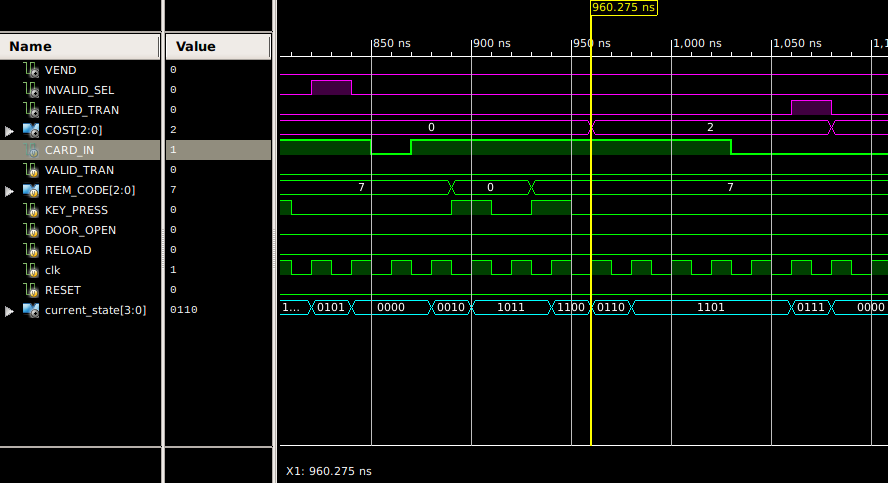
\includegraphics[scale=0.45]{waveform-5.png} \\
        \caption{Simulation Waveform for Case 5}
    \end{center}
    
    \item \textbf{Unsuccessful Purchase, Door Does Not Open}   \\
    This case represents an unsuccessful purchase where valid keys are inputted, and the transaction is valid, but the door of vending machine does not open. To simulate this case, we set \texttt{CARD\_IN = 1} to transition into state \texttt{4'b0010} CARD\_INSERT\_WAIT, we then set \texttt{KEY\_PRESS = 1} for one cycle, and then set \texttt{KEY\_PRESS = 1} for one cycle. From diagram below, we can see that we entered the key 0 and then the key 2, which is a valid item with stock as the machine was reloaded previously. Thus, we see that output \texttt{COST} is correctly 2. At 1240ns, the \texttt{VALID\_TRAN} signal is detected by our FSM, so output \texttt{VEND = 1}. From 1240ns on, we are in the state where we're waiting for either door to open or 5 cycles to pass. At 1340ns, 5 cycles has passed and door did not open, so we set all output to 0 and return to IDLE state. 
    \begin{center}
        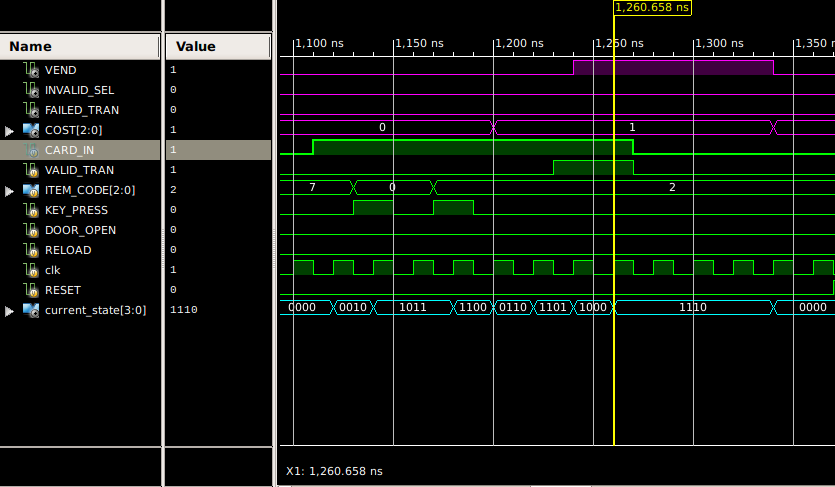
\includegraphics[scale=0.5]{waveform-6.png} \\
        \caption{Simulation Waveform for Case 6}
    \end{center}
    
    \item \textbf{Unsuccessful Purchase, Valid Input, No Stock}   \\
    This case represents an unsuccessful purchase where valid keys are inputted, but because we have no more stock of the requested item left, we set \texttt{INVALID\_SEL = 1} and return to IDLE state.  To simulate this case, we have to first make sure there is no more stock of a particular item. To do this, we set input \texttt{RESET = 1} for one cycle to make sure all counts of our item is 0. We then set \texttt{CARD\_IN = 1} to transition into state \texttt{4'b0010} CARD\_INSERT\_WAIT, we then set \texttt{KEY\_PRESS = 1} for one cycle, and then set \texttt{KEY\_PRESS = 1} for one cycle. From diagram below, we can see that we entered the key 1 and then the key 3, which is a valid item number as it is within 00-19. But since our vending machine is out of stock, we can see that at 1500ns, \texttt{INVALID\_SEL = 1} for one cycle after second key is entered. This is the correct expected behavior. All other outputs remain correctly at 0.
    \begin{center}
        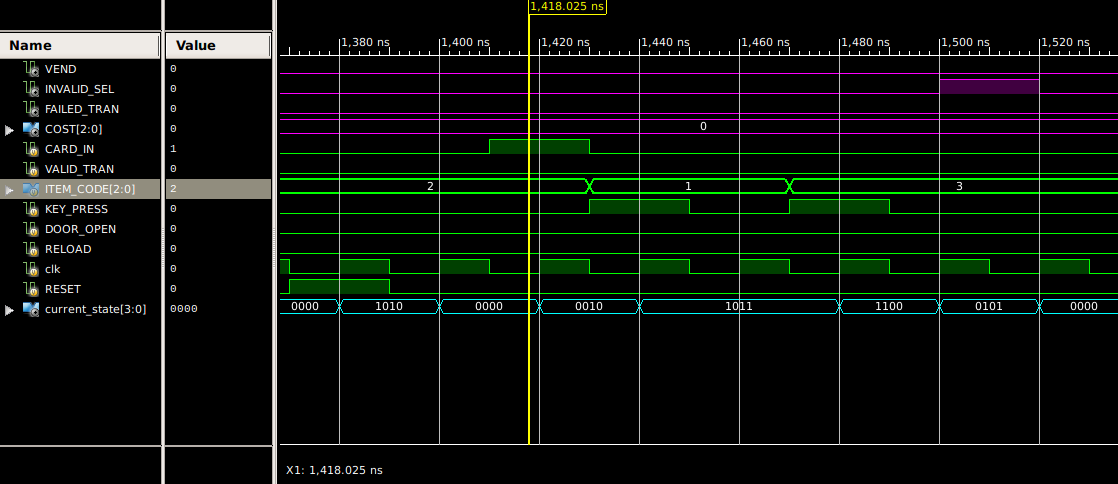
\includegraphics[scale=0.4]{waveform-7.png} \\
        \caption{Simulation Waveform for Case 7}
    \end{center}
    \item \textbf{Case Where Signals Change} \\ \\
    This case occurs throughout the waveform diagrams above as often the \texttt{CARD\_IN} signal stays high throughout transaction or goes low in the middle of a transaction. We can see that we correctly handle this case as regardless of how long \texttt{CARD\_IN} signal stays high, our module treats it correctly. If card is taken out earlier, it is okay, as our vending machine remembers the card info. So no odd behavior will happen when signals change arbitrarily.
\end{enumerate}
One bug I found during simulation for this project was that my counter that keeps track of whether 5 cycle has passed was incorrect, as it continues to count up even in cases where the counter is not needed. I fixed this by adding an additional internal register to signal when count should be incremented.

\section{Synthesis and Implementation Report}
Sections of Synthesis and Implementation Report is attached at end of report.  From the 'Design Summary' part of the synthesis report, we can conclude the different components that my implementation of the Vending Machine FSM uses. For example, we can see that we indeed do use a lot of registers from the synthesis report and we can also see the different clock signals needed for our module. From implementation report, we can see that there is no errors when trying to implement our module, but there are a few warnings due to truncation of numbers into registers. The warnings can be ignored as in my code I made sure that truncation will not occur for those registers.

\section{Conclusion} 
In this project, I designed and implemented the Vending Machine FSM according to the behavior in the project manuscript. I designed the Vending Machine based on a Moore Machine, that has similar structure to the turnstile FSM example in the manuscript. To correctly implement this, I had to first draw the FSM diagram to allow me to clearly see what output should be in each state and how to transition to a different state. One of the major difficulty I encountered in this assignment was trying to incorporate a counter in order to keep track of whether 5 cycles has passed. I dealt with this by experimenting my code on a smaller, simpler module in order to see how to correctly use different signal within my module to signal counter to start counting and to detect output of the counter. 

\newpage
\small
\section{Reports}
\subsection{Synthesis Report}
\verbatiminput{syn-report-lab4.txt}
\newpage
\subsection{Implementation Report}
\verbatiminput{imp-report-lab4.txt}

\end{document}